\chapter{Concept Description}
The project's goal is the construction of a platform that facilitates the communication and authorization aspects of remote controlling a device over the internet.
Agents connect to the platform through which their sensory information, available commands and functions are made available to authorized users.
Use of the platform increases the possible simultaneous audience of a connected agent, as users do not have to query the agent directly for the information. 
Agents actively query the platform to obtain commands from users.
In the same manner, users must actively query the platform to obtain new information from or about the agents.
The frequency of such queries are decided by the specific client.
See Figure \ref{fig:system-overview} for an illustration of the flow of information between the platform and connected entities.

\begin{figure}[H]
\begin{center}
	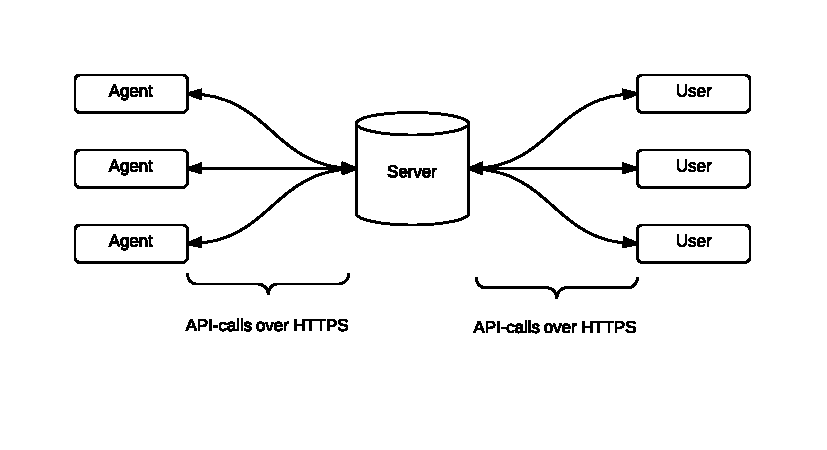
\includegraphics{graphics/system-overview.pdf}
	\caption{An overview of the concept showing three users and three agents communicating through the platform.}
	\label{fig:system-overview}
\end{center}
\end{figure}

The platform itself only responds to queries from connected entities and performs user identification and authentication if needed.
When a user sends a command to an agent, the command is received by the server and is stored away until the agent queries the platform for commands directed at it.
When an agent uploads its sensor data or whatever other information this is stored on the platform and users must actively query the platform for it.

Agents and users access the platform through a client, which is a piece of software that communicates with the platform.
On the user side, the client communicates with the platform through API calls and presents the information it receives to the user.
On the agent side, the client communicates with the platform through API calls, and translates (if required) and passes this information on to the device that is to be remote controlled.
Clients are not a part of the platform itself, and the only requirement is that they are able to communicate with the platform through the API.

\section{Terminology}
% Terminology!
Below follows an explanation of the various words that refer to different parts of the system.

\paragraph{Server} the physical computer or cluster of computers on which the service is hosted.

\paragraph{Service} the program that facilitates the communication between clients and manages user authentication.

\paragraph{Platform} see Service.

\paragraph{Client} any software that sends requests to the service and receives the responses.

\paragraph{Agent} any entity that is connected to the service that can receive commands through the service.
The term ``agent'' refers to the entire entity, which is considered to begin where the requests to the service are generated and end wherever the commands are acted out.
A robot, its actuators and sensors, the software that communicates with the service, and the computer that is connected to the robot which the software runs on, and any other parts or components are considered part of the agent.

\paragraph{User} any non-agent entity that interacts with the service.
This includes actual people and automated services -- anything that interacts with the service but cannot receive commands through it.

\paragraph{User client} any client that allows users access to the service.



